\chapter{The moving frame}\label{chapter:moving.frame}%
\chapterSummary{%
In most chapters of these notes, we study geometry that is invariant under diffeomorphisms.
In this chapter, we study geometry that is invariant under rigid motions of \(3\)-dimensional Euclidean space.}

\section{Notation}
\emph{Warning}: We use the notation \(\E[3]\) instead of \(\R[3]\) to mean Euclidean space, i.e. \(\R[3]\) with its usual metric.

\medskip

\par\noindent
\emph{Warning}: In this chapter, \(e_1, e_2, e_3\) is \emph{not} necessarily the standard basis of \(\E[3]\); it is an arbitrary orthonormal basis.

\section{Orthonormal frames}
An \emph{orthonormal frame}\define{orthonormal frame}\define{frame!orthonormal} is a pair \((x,e)\) where \(x \in \E[3]\) and 
\[
 e=\pr{e_1 \ e_2 \ e_3}
\]
is an orthonormal basis of \(\E[3]\) arranged into the columns of a matrix.
\begin{center}
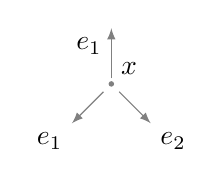
\begin{tikzpicture}
\fill [gray] (0,0) circle (1pt) node[black,above right]{\(x\)};
\draw[-latex,gray] (0,.07071) -- (0,.7071) node[black,below left]{\(e_1\)};
\draw[-latex,gray] (-.1,-.1) -- (-.5,-.5) node[black,below left]{\(e_1\)};
\draw[-latex,gray] (.1,-.1) -- (.5,-.5) node[black,below right]{\(e_2\)};
\end{tikzpicture}
\end{center}
\begin{problem}{moving.frame:rigid}
For any two frames \((x,e), \pr{x',e'}\), there is a unique rigid motion \(\phi\), i.e. a distance preserving transformation, taking one to the other: \(x'=\phi(x)\), \(e'_i=\phi_* e_i\).
\end{problem}
Each rigid motion \(\phi\) has associated frame \((x,e)\) which is the frame that arises when we apply \(\phi\) to the standard basis frame at the origin.
Let \(\Orth{3}\) be the set of \(3 \times 3\) orthogonal matrices.
To each orthonormal frame \((x,e)\in\frameBundleE{3}\), associate the matrix
\[
h=
\begin{pmatrix}
1 & 0 \\
x & e
\end{pmatrix}
\]
giving a map
\[
h \colon (x,e) \in \frameBundleE{3}\mapsto h(x,e) \in \E[3] \ltimes \Orth{3}.
\]
\begin{problem}{moving.frame:isom}
Prove that: associating to \(\phi\) this matrix \(h(x,e)\) above is an isomorphism of groups from the group of rigid motions of Euclidean space to the group \(\Orth{3} \ltimes \E[3]\) of such matrices.
So \(h(x,e)\) ``is'' the rigid motion that takes the origin to \(x\) and the standard basis to \(e\).
Prove that
\[
h(x,eg)=h(x,e)
\begin{pmatrix}
1 & 0 \\
0 & g
\end{pmatrix}
\]
for any orthogonal \(3 \times 3\) matrix \(g\).
\end{problem}

\section{Frames on curves}
Take a curve in \(\E[3]\)
\begin{center}
\input{curve}
\end{center}
and consider all of the frames \((x,e)\) with \(x\) a point of the curve.
\begin{center}
\documentclass[tikz]{standalone}
\usetikzlibrary{hobby, arrows.meta,bending,decorations.markings}
\begin{document}
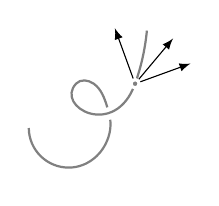
\begin{tikzpicture}[baseline,scale=.75]
\draw[gray,thick] (.1,.85) to [curve through={(.79,.18) .. (1.45,.7) (1.48,.99) .. ([blank=soft]1.43,1.2) .. (1.2,1.6) .. (.9,1.6) .. (1.9,1.6)}] (2.1,2.5);
\draw[-latex] (1.9,1.6) -- ({1.9+cos(20)},{1.6+sin(20)});
\draw[-latex] (1.9,1.6) -- ({1.9+cos(50)},{1.6+sin(50)});
\draw[-latex] (1.9,1.6) -- ({1.9+cos(110)},{1.6+sin(110)});
\fill[gray,draw=white,very thick] (1.9,1.6) circle (2pt);
\end{tikzpicture}
\end{document}

\end{center}
At each point \(x\) of the curve, any two such frames agree up to orthogonal transformation; the set of all such frames is a \(4\)-dimensional manifold.
If a rigid motion takes one curve to another, it takes these frames along the one curve to those along the other curve.
If the curve is immersed, a frame \((x,e)\) is \emph{adapted} if \(e_1\) is tangent to the curve.
\begin{center}
\documentclass[tikz]{standalone}
\usetikzlibrary{hobby, arrows.meta,bending,decorations.markings}
\begin{document}
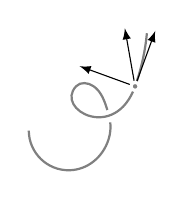
\begin{tikzpicture}[baseline,scale=.75]
\draw[gray,thick] (.1,.85) to [curve through={(.79,.18) .. (1.45,.7) (1.48,.99) .. ([blank=soft]1.43,1.2) .. (1.2,1.6) .. (.9,1.6) .. (1.9,1.6)}] (2.1,2.5);
%\draw[thick,-stealth] (1.9,1.6) -- ({1.9+cos(20)},{1.6+sin(20)});
%\draw[thick,-stealth] (1.9,1.6) -- ({1.9+cos(50)},{1.6+sin(50)});
%\draw[thick,-stealth] (1.9,1.6) -- ({1.9+cos(110)},{1.6+sin(110)});
\draw[-latex] (1.9,1.6) -- ({1.9+cos(70)},{1.6+sin(70)});
\draw[-latex] (1.9,1.6) -- ({1.9+cos(100)},{1.6+sin(100)});
\draw[-latex] (1.9,1.6) -- ({1.9+cos(160)},{1.6+sin(160)});
\fill[gray,draw=white,very thick] (1.9,1.6) circle (2pt);
\end{tikzpicture}
\end{document}

\end{center}
At each point \(x\) of the curve, any two adapted frames agree up to changing the direction of \(e_1\), and rotating or reflecting \(e_2,e_3\) in the plane normal to the tangent line; the set of all such frames is a surface inside that \(4\)-dimensional manifold.
This surface of adapted frames is built by attaching to each point of \(C\) four circles, representing rotating \(e_2,e_3\)  and reflecting \(e_1\) or the plane or \(e_2,e_3\).
We will carry out computations directly inside that surface.
On a connected curve, that surface has \(4\) components.
Every rigid motion is determined by where it moves any chosen frame.
Any rigid motion preserving an immersed curve takes any frame adapted to the curve to another frame adapted to the curve.
So we can guess that the group of rigid motions preserving an immersed curve is at most a \(2\)-dimensional submanifold of the \(6\)-dimensional group of rigid motions.

\section{Frames on surfaces}
Similarly, a frame is adapted to a surface if \(e_3\) is normal to the surface.
\begin{center}
\documentclass[tikz]{standalone}
\begin{document}
\begin{tikzpicture}
\node[anchor=south west,inner sep=0] at (0,0) {\includegraphics[width=.5\textwidth]{genus-2-surface-2.pdf}};
\draw[gray,thick,-stealth] (1.5,2.3) -- ({1.5+cos(20)},{2.3+sin(20)});
\draw[gray,thick,-stealth] (1.5,2.3) -- ({1.5+cos(-30)},{2.3+sin(-30)});
\draw[gray,thick,-stealth] (1.5,2.3) -- ({1.5+cos(90)},{2.3+sin(90)});
\fill[gray,thick] (1.5,2.3) circle (1pt);
\end{tikzpicture}
\end{document}
\end{center}
The set of adapted frames \((x,e)\) of a surface is a \(3\)-dimensional manifold, as we can move the point \(x\) along the surface, and rotate \(e_1,e_2\) around \(e_3\).
Hence the group of rigid motions preserving an immersed surface is at most a \(3\)-dimensional submanifold of the \(6\)-dimensional group of rigid motions.

\section{The frame bundle}
The \emph{frame bundle}\define{frame bundle}\define{bundle!frame} \(\frameBundleE{3}\) of Euclidean space \(\E[3]\) is the set of all orthonormal frames. 
Any rigid motion \(\phi\) of \(\E[3]\) takes \(e_1, e_2, e_3\) to \(\phi_* e_1, \phi_* e_2, \phi_* e_3\).
If you pick an orthonormal frame \((x,e)\) and I pick another one, say \((x,e')\) at the same point \(x\), then yours and mine must agree up to a unique orthogonal matrix, because they are orthonormal bases of the same vector space \(\E[3]\).
So \(e_j' = \sum_i g_{ij} e_i\) for a uniquely determined orthogonal \(3 \times 3\) matrix \(g=\pr{g_{ij}}\); denote this \(e'\) as \(eg\).
An orthonormal frame \((x,e)\) with \(e=(e_1 \ e_2 \ e_3)\) has \(e \in \Orth{3}\) an orthogonal matrix,  so \(\frameBundleE{3}=\E[3] \times \Orth{3}\) and the expression \(eg\) is matrix multiplication.

\section{Adapted frames for a curve}
Take a curve \(C\) in \(\E[3]\).
At each point \(c \in C\), take \(e_1\) to be a unit vector tangent to \(C\).
We can pick an adapted frame \((x,e)\), uniquely up to replacing \((x,e)\) by \((x,eg)\) for any orthogonal matrix
\[
g=
\begin{pmatrix}
\pm1&0\\
0&h
\end{pmatrix},
h\in\Orth{2}.
\]
The \emph{curvature vector}%
\define{curvature vector}  of \(C\) at a point is the acceleration as we move along \(C\) at unit speed.
If we change the choice of unit speed parameterization (also known as \emph{arclength parameterization}, adding a constant or changing the direction of motion, i.e. the sign, this changes the sign of velocity, but we hit two sign changes when we take two derivatives, so the curvature vector is independent of the choice of unit speed parameterization.
In particular, the curvature vector is defined without selecting any orientation of the curve \(C\).

Write the (perhaps local) inverse of an arclength parameterization as a function \(s\) on an open subset of \(C\), uniquely determined up to sign and adding a constant.
The identity function \(x \mapsto x\) on \(\E[3]\) restricts to a function \(x \colon C \to \E[3]\), and clearly
\[
e_1 = \frac{dx}{ds},
\]
when we take \(e_1\) to point in the direction of increasing \(s\), i.e. use \(s\) to orient \(C\).
Differentiating again, the curvature vector of \(C\) is 
\[
\kappa \defeq \frac{de_1}{ds}.
\]
If \(\kappa = 0\) at every point of the curve then the curve is a straight line.
If \(\kappa \ne 0\) at some point, then we can uniquely determine a unit normal vector \(e_2\) to \(C\) by
\[
e_2 \defeq \frac{\kappa}{\norm{\kappa}},
\]
and then define the \emph{curvature} to be \(k\defeq \norm{\kappa}\).
Having chosen \(e_1,e_2\) at each point of our curve, \(e_3\) is determined up to sign, and can be chosen smoothly.
\begin{problem}{moving.frame:derive.S.F}
Calculate that
\[
\frac{de_2}{ds}  = - k e_1 + t e_3, \quad \frac{de_3}{dt} = -te_2,
\]
for some function \(t\),  the \emph{torsion}.\define{torsion!of a curve}
\end{problem}
The sign of \(t\) depends on the choice of \(e_3\), which is unique up to sign, so \(te_3\) is defined independent of choice of \(e_3\).
But \(te_3\) still depends on the choice of sign of \(e_1\), i.e. the direction of motion.
So we could say that the complicated expression \(te_3 \, ds\), a \(1\)-form valued in the normal line to the curve, is an invariant independent of any choices.
\begin{answer}{moving.frame:derive.S.F}
Since \(e\) is orthogonal, its transpose is \(\transpose{e}=e^{-1}\), i.e. \(\transpose{e}e=I\), i.e. \(e_i \cdot e_j=1\) if \(i=j\), \(0\) otherwise.
Differentiate: \(\transpose{\dot{e}} e + \transpose{e} \dot{e}=0\), i.e. \(\transpose{e}\dot{e}=-\transpose{\dot{e}}e=-\transpose{(\transpose{e}\dot{e})}\), i.e. \(\transpose{e}\dot{e}\) is antisymmetric, with entries \(e_i \cdot \dot{e}_j\).
Since \(\dot{e}_1=ke_2\),
\[
\transpose{e}\dot{e}=
\begin{pmatrix}
0 & ? & ? \\
k & ? & ? \\
0 & ? & ?
\end{pmatrix}.
\]
By antisymmetry,
\[
\transpose{e}\dot{e}=
\begin{pmatrix}
0 & -k & 0 \\
k & 0 & -t \\
0 & t & 0
\end{pmatrix}
\]
for some \(t\).
\end{answer}
The frame \(e_1, e_2, e_3\) of an oriented curve of nonzero curvature is the \emph{Serret--Frenet frame}\define{Serret--Frenet frame}.
Note that we can change sign of \(e_1\), i.e. change orientation, and independently change sign of \(e_3\).
So the frame bundle of \(C\) contains four Serret--Frenet frames above each point of \(C\), i.e. four curves in the frame bundle.
The torsion changes sign if we change the sign of \(e_3\), so it is not really a function on the curve \(C\).
We can pick out one choice of Serret--Frenet curve by orienting both \(C\) and \(\E[3]\).
We can guess that the isometries of \(\E[3]\) which preserve a nonlinear curve are at most \(1\)-dimensional.
\begin{problem}{moving.frame:torsion}
For a curve with nonzero curvature vector, prove that its torsion vanishes if and only if the curve lies in a plane.
\end{problem}
\begin{example}
Intuitively, torsion controls the rate at which the curve twists out of its tangent plane, while the curvature controls the rate at which the curve twists in its tangent plane.
\end{example}
\begin{example}
With only rigid motions, we can turn a circle around, slide a line along itself, and twist a helix\SubIndex{helix} along itself, and allow reflections in direction.
The adapted frames of these curves are taken one to another by these rigid motions.
So the curvature and torsion functions are constant, except that the torsion changes sign if we change the choice of \(e_3\), or of direction of motion along the curve.
\end{example}
\begin{problem}{moving.frame:helix}
Compute the curvature and torsion of a helix.
Prove that any constant values of curvature and torsion can arise for a suitable choice of helix.
\end{problem}
\begin{answer}{moving.frame:helix}
For any constants \(\alpha,\beta,\gamma\), let
\[
\begin{pmatrix}
x_1\\
x_2\\
x_3
\end{pmatrix}
\defeq
\begin{pmatrix}
\alpha \cos \beta s \\
\alpha \sin \beta s\\
\gamma s
\end{pmatrix}.
\]
so
\[
\begin{pmatrix}
\dot{x}_1\\
\dot{x}_2\\
\dot{x}_3
\end{pmatrix}
=
\begin{pmatrix}
-\alpha\beta \sin \beta s \\
\alpha \beta \cos \beta s\\
\gamma
\end{pmatrix},
\]
\[
\norm{\dot{x}}^2=\alpha^2\beta^2+\gamma^2.
\]
So we need this to equal \(1\).
Clearly \(\alpha=0\) or \(\beta=0\) is a line, and \(\gamma=0\) is a circle.
We ignore those cases and so the equation \(\alpha^2\beta^2+\gamma^2=1\) can be solved for any of these three constants in terms of the other two.
We can reflect in the \(x_1x_2\) plane to arrange that \(\alpha,\beta>0\) and in the \(x_3\) axis to arrange that \(\gamma>0\).
We get
\[
e_1
=
\begin{pmatrix}
-\alpha\beta \sin \beta s \\
\alpha \beta \cos \beta s\\
\gamma
\end{pmatrix}
\]
so
\[
\dot{e}_1=ke_2=
\begin{pmatrix}
-\alpha\beta^2 \cos \beta s \\
-\alpha \beta^2 \sin \beta s\\
0
\end{pmatrix},
\]
so
\[
k=\alpha\beta^2
\]
and
\[
e_2=
-
\begin{pmatrix}
\cos \beta s \\
\sin \beta s\\
0
\end{pmatrix}.
\]
Differentiate
\[
\dot{e}_2
=
\begin{pmatrix}
\beta\sin \beta s \\
-\beta\cos \beta s\\
0
\end{pmatrix}
\]
so
\[
te_3=\dot{e}_2+ke_1=te_3
=
\begin{pmatrix}
\beta\gamma^2\sin \beta s\\
-\beta\gamma^2\cos \beta s\\
\alpha\beta^2\gamma
\end{pmatrix}.
\]
Finally,
\[
t=\pm\beta\gamma,
\]
and
\[
e_3=
\pm
\begin{pmatrix}
\gamma\sin \beta s\\
-\gamma\cos \beta s\\
\alpha\beta
\end{pmatrix}.
\]
So if we set 
\begin{align*}
\beta\defeq\sqrt{k^2+t^2},\\
\alpha\defeq\frac{k}{\beta^2},\\
\gamma\defeq\pm\frac{t}{\beta},
\end{align*}
we get a helix with prescribed constant values of \(k,t\).
\end{answer}
\begin{theorem}
Take an interval \(I \subset \R\).
Given a continuous positive function \(k \colon I \to (0,\infty)\) and a continuous function \(t \colon I \to \R\), there is a curve \(C\) in \(\E[3]\) with twice continuously differentiable unit speed parameterization \(x \colon I \to \E[3]\) and with curvature \(k\) and torsion \(t\).
Any two such curves are identified by a unique rigid motion of \(\E[3]\).
\end{theorem}
\begin{proof}
To each adapted frame \((x \ e)\), associate the matrix
\[
g=
\begin{pmatrix}
1 & 0 \\
x & e
\end{pmatrix}.
\]
This \(g\) maps each adapted frame \((x \ e)\) of the curve to the rigid motion \(g(x \ e)\) which takes the origin to \(x\) and the standard basis to \(e\).
For the adapted frames of a curve, the above gives
\[
\frac{dg}{ds} = 
g
\begin{pmatrix}
0 & 0 & 0 & 0 \\
1 & 0 & -k & 0 \\
0 & k & 0 & -t \\
0 & 0 & t & 0
\end{pmatrix}.
\]
These equations are linear, so there are global continuously differentiable solutions, by the existence and uniqueness theorem for linear ordinary differential equations, with any initial data.
Expand out to
\begin{align*}
\frac{dx}{ds} &= e_1, \\
\frac{d}{ds}
\begin{pmatrix}
e_1 & e_2 & e_3
\end{pmatrix}
&=
\begin{pmatrix}
e_1 & e_2 & e_3
\end{pmatrix}
\begin{pmatrix}
0 & -k & 0 \\
k & 0 & -t \\
0 & t & 0
\end{pmatrix}
\end{align*}
If \(e_1, e_2, e_3\) are orthonormal at one point \(s_0 \in I\), then
\[
\frac{d}{ds} e_1 \cdot e_1
=
2 e_1 \cdot k e_2 = 0,
\]
etc., so remains an orthonormal frame.
The choice of initial conditions at a single point determines the curve and the frame.
If we translate \(x\) or rotate \(x,e_1,e_2,e_3\) by a constant rotation, check that this takes us to another solution.
Since \(e_1(s)\) is continuously differentiable and \(dx/ds=e_1\), \(x\) is twice continuously differentiable. 
\end{proof}
\begin{example} Any curve of constant positive curvature and constant nonzero torsion is a helix, by existence (from the problem above) and uniqueness.
Similarly, any curve of constant positive curvature and zero torsion is a circle, and any curve of zero curvature is a line.
\end{example}
\begin{problem}{moving.frame:Bertrand}
For a given curve in \(3\)-dimensional Euclidean space, with nowhere vanishing curvature vector, find every other curve so that, parameterized by arc length, points with the same arclength parameter have the same direction of curvature vector.
\end{problem}
\begin{answer}{moving.frame:Bertrand}
If \(\ot{e}_2=e_2\), then \(e_1,e_3\) and \(\ot{e}_1,\ot{e}_3\) are orthonormal bases of the same plane \(e_2^{\perp}\).
Choose the sign of \(e_3\) to get 
\[
\ot{e}_1+i\ot{e}_3=e^{i\theta}(e_1+ie_3)
\]
for some angle \(\theta\).
Differentiate to get
\[
d\ot{e}_1+i \, d\ot{e}_3=\dot\theta e^{i\theta}(e_1+ie_3)+e^{i\theta}(\dot{e}_1+i\dot{e}_3).
\]
Expand to get
\[
(\ot{k}-i\ot{t})e_2=\dot\theta e^{i\theta}(e_1+ie_3)+e^{i\theta}(k-it)e_2
\]
Differentiate \(e_2=\ot{e}_2\) to get \(-\ot{k}\ot{e}_1+\ot{t}\ot{e}_3=-ke_1+te_3\).
Hence
\[
\ot{k}+i\ot{t}=e^{-i\theta}(k+it).
\]
So \(\dot\theta=0\), a constant rotation.

On the other hand, we can now pick any constant \(\theta\), and define:
\begin{align*}
\ot{e}_1+i\ot{e}_3\defeq e^{i\theta}(e_1+ie_3), \\
\ot{e}_2\defeq e_2,\\
\ot{k}+i\ot{t}\defeq e^{-i\theta}(k+it),\\
\ot{x}=\int \ot{e}_1 \, ds
\end{align*}
and check that the Serret--Frenet equations are satisfied, so these yield the Serret--Frenet frame of a curve.
\end{answer}

\section{Adapted frames for a surface}
An \emph{adapted orthonormal frame}% 
\define{frame}
(or just \emph{frame} for short) on a surface \(S\) in \(\E[3]\) is an orthonormal frame \((x,e) \in \frameBundleE{3}\) so that \(x \in S\) and \(e_1, e_2\) are tangent to \(S\) at \(x\), and therefore \(e_3\) is normal to \(S\).
\begin{example} 
If \(S\) is the unit sphere in \(\E[3]\), we can write the points of \(S\) as
\[
x
=
\begin{pmatrix}
x_1 \\
x_2 \\
x_3
\end{pmatrix}
\]
with \(1=x_1^2+x_2^2+x_3^2\).
Away from the north or south pole, we can take
\[
e_1
=
\frac{1}{\sqrt{x_1^2+x_3^2}}
\begin{pmatrix}
x_3 \\
0 \\
-x_1
\end{pmatrix},
e_2
=
\frac{1}{\sqrt{x_1^2+x_3^2}}
\begin{pmatrix}
x_1 x_2 \\
-\pr{x_1^2+x_3^2} \\
x_2 x_3
\end{pmatrix}
\]
tangent and 
\[
 e_3=
 \begin{pmatrix}
  x_1 \\
  x_2 \\
  x_3
 \end{pmatrix}
\]
normal.
We can choose \(e_3\) to point outward from \(S\) in either direction, and choose \(e_1, e_2\) to have either orientation.
\end{example}
The \emph{frame bundle}%
\define{frame!bundle}
\(\frameBundle{S}\) is the set of all adapted orthonormal frames for \(S\).
The manifold \(\frameBundle{S}\) is a \(3\)-dimensional submanifold of \(\frameBundleE{3}=\E[3] \times \Orth{3}\).
\begin{problem}{moving-frame:sphere.frame.bundle}
Explain why, if \(S=\mathbb{S}^2 \subset \E[3]\) is the unit sphere around the origin, then \(\frameBundle{S}\) is diffeomorphic to two disjoint copies of \(\Orth{3}\), given by the equation \(x=\pm e_3\).
\end{problem}
The subgroup \(\Orth{2} \times \pm 1 \subset \Orth{3}\) of orthogonal linear transformations of \(\E[2]\) and \(\E[1]\) acts on \(\frameBundle{S}\) as \((x,e)g=(x,eg)\) where 
\[
 g=\begin{pmatrix}
    h & 0 \\
    0 & n
   \end{pmatrix}
\]
with \(h \in \Orth{2}\) and \(n\in\Orth{1}=\{\pm 1\}\).

\section{The soldering forms}
If \(v\) is a tangent vector on the manifold \(\frameBundleE{3}\), we can write \(v\) as \(\pr{\dot{x},\dot{e}}\), an infinitesimal motion \(\dot{x}\) of the point \(x\), and an infinitesimal rotation \(\dot{e}\) of the frame \(e\).
We can write out any tangent vector \(\dot{x}\) in terms of the basis \(e_1, e_2, e_3\), say as \(\dot{x} = a_1 e_1 + a_2 e_2 + a_3 e_3\).
The \emph{soldering forms}\define{form!soldering}\define{soldering forms} are the \(1\)-forms \(\omega_1, \omega_2, \omega_3\) on \(\frameBundleE{3}\) given by \(\pr{\dot{x},\dot{e}} \hook \omega_i = a_i\).
So the soldering forms measure, as we move a frame, how the base point of the frame moves, as measured in the frame itself as a basis.

The \emph{identity function} on \(\E[3]\), which we write as \(x\), is defined as \(x(p)=p\) for any point \(p \in \E[3]\).
Of course \(dx(v)=v\) for any vector \(v\), i.e. \(dx=I\) is the identity matrix.
We define \(x\) also on \(\frameBundleE{3}\) by \(x(p,e)=p\).
We can write the \(1\)-forms \(\omega_1, \omega_2, \omega_3\) on \(\frameBundleE{3}\) as \(\omega_1=e_1 \cdot dx, \omega_2=e_2 \cdot dx, \omega_3=e_3 \cdot dx\).
On our vector \(v=\pr{\dot{x},\dot{e}}\), we have \(v \hook \omega_i=e_i \cdot \dot{x}=a_i\).


\section{The connection forms}
When we move a frame \((x,e)\), the soldering forms measure the motion of the underlying point \(x\).
We want to measure the rotation of the vectors \(e_1, e_2, e_3\).
Infinitesimal rotations are complicated.
Write the inner product on \(\E[3]\) as \(x \cdot y=x_1 y_1 + x_2 y_2 + x_3 y_3\). 
So
\[
e_i \cdot e_j=
\begin{cases}
1 & \text{if \(i=j\)}, \\
0 & \text{if \(i\ne j\)}.
\end{cases}
\]
If we rotate an orthonormal basis \(e_1, e_2, e_3\) through a family of orthonormal bases \(e_1(t), e_2(t), e_3(t)\), along some curve \(x(t)\), these still have the same constant values of \(e_i(t) \cdot e_j(t)\) at every time \(t\).
Differentiate: \(0=\dot{e}_i(t) \cdot e_j(t) + e_i(t) \cdot \dot{e}_j(t)\).
Therefore we can write any infinitesimal rotation of frame as \(\dot{e}_j = \sum_i a_{ij} e_i\) for an antisymmetric \(3 \times 3\) matrix \(A=\pr{a_{ij}}\).
The quantity \(a_{ij}\) measures how quickly \(e_j\) is moving toward \(e_i\).

The \emph{Levi-Civita connection forms}\define{connection forms!Levi-Civita}\define{Levi-Civita connection!forms} are the \(1\)-forms \(\gamma_{ij}=e_i \cdot de_j\), i.e. \(v \hook \gamma_{ij} = a_{ij}\): so \(\gamma_{ij}\) measures the tendency of \(e_j\) to move toward \(e_i\) as the frame moves.
In particular, \(0=\gamma_{ij}+\gamma_{ji}\).
These \(\omega_i\) and \(\gamma_{ij}\) are defined on \(\frameBundleE{3}\), \emph{not} on \(\E[3]\), because they depend on \(x\) and \(e\).
If we move a frame, we said it moves by a velocity vector \(v=\pr{\dot{x},\dot{e}}\) with \(\dot{e}_i = \sum_j a_{ji} e_j\) for an antisymmetric matrix \(a_{ij}\), so
\[
v \hook \gamma_{ij} = v \hook e_i \cdot de_j = e_i \cdot \dot{e}_j = a_{ij}.
\]
So the \(1\)-forms \(\omega_i\) restrict to any ``moving frame'' \(\pr{x(t),e(t)}\) to describe how the velocity of the moving point \(x(t)\) is expressed in the moving frame \(e(t)\), while the \(1\)-forms \(\gamma_{ij}\) describe how the infinitesimal rotation of the moving frame \(e(t)\) is expressed at each moment in the moving frame \(e(t)\).

Write our soldering forms as \(\omega\), thought of as a column of \(1\)-forms
\[
\omega
=
\begin{pmatrix}
\omega_1 \\
\omega_2 \\
\omega_3
\end{pmatrix}
\]
and our connection \(1\)-forms as
\[
\gamma=
\begin{pmatrix}
\gamma_{11} & \gamma_{12} & \gamma_{13} \\
\gamma_{21} & \gamma_{22} & \gamma_{23} \\
\gamma_{31} & \gamma_{32} & \gamma_{33} 
\end{pmatrix}
=
\begin{pmatrix}
0 & \gamma_{12} & \gamma_{13} \\
-\gamma_{12} & 0 & \gamma_{23} \\
-\gamma_{13} & -\gamma_{23} & 0
\end{pmatrix}
\]
an antisymmetric matrix of \(1\)-forms, the \emph{Levi-Civita connection}.

\begin{problem}{moving.frame:derive.structure.equations}
Prove that the soldering and Levi-Civita connection forms satisfying the \emph{structure equations of Euclidean space}:\define{structure equations!of Euclidean space}
\begin{align*}
d \omega_i &= - \sum_j \gamma_{ij} \wedge \omega_j, \\
d \gamma_{ij} &= -\sum_k \gamma_{ik} \wedge \gamma_{kj}.
\end{align*}
\end{problem}
\begin{answer}{moving.frame:derive.structure.equations}
The proof requires some unwinding of notation: the expression \(\omega_i=e_i \cdot dx\) means that \(\omega_i = \sum_j e_{ji} dx_j\), which allows us to unwind the following formal steps:
\begin{align*}
d\omega_i &= d\pr{e_i \cdot dx},\\
&= de_i \wedge dx, \\
&= \sum_j \pr{e_j \cdot de_i} \wedge \pr{e_j \cdot dx}, \\
&= \sum_j \gamma_{ji} \wedge \omega_j.
\end{align*}
Similarly, the expression \(\gamma_{ij}=e_i \cdot de_j\) means that \(\gamma_{ij} = \sum_k e_{ki} de_{kj}\), so:
\begin{align*}
d\gamma_{ij} &= d\pr{e_i \cdot de_j}, \\
&= de_i \wedge de_j, \\
&= \sum_k \pr{e_k \cdot de_i} \wedge \pr{e_k \cdot de_j}, \\
&= \sum_k \gamma_{ki} \wedge \gamma_{kj}.
\end{align*}
\end{answer}

\begin{problem}{moving.frame:structure.group.action}
For \(g\) any \(3 \times 3\) orthogonal matrix, if we write \(r_g(x,e)\) to mean \((x,eg)\), and \(\transpose{g}\) for the transpose of \(g\), prove that \(r_g^* \omega=\transpose{g}\omega\) and \(r_g^* \gamma = \transpose{g}\gamma g\).
Expanding out, this means \(r_g^*\omega_i = \sum_j g_{ji} \omega_j\) and \(r_g^*\gamma_{ij} = \sum_{k\ell} g_{ki} \gamma_{k\ell} g_{\ell j}\).
\end{problem}
\begin{answer}{moving.frame:structure.group.action}
Here are two proofs:
\begin{enumerate}
\item
If we think of \(x\) and \(e\) as functions on \(\frameBundleE{3}\), then \(r_g^* x = x\), \(r_g^* e = eg\).
Hence \(r_g^* dx=dx\) and \(r_g^* de = (de)g\).
So \(r_g^* \omega = r_g^* (\transpose{e}\, dx)= \transpose{(eg)} dx = \transpose{g} \transpose{e} dx = \transpose{g} \omega\) and \(r_g^*\gamma = r_g^* (\transpose{e} de) = \transpose{(eg)} d(eg)=\transpose{g} \transpose{e} de \, g=\transpose{g} \gamma g\).
\item
The action is \(r_g(x,e)=(x,eg)\), where \((eg)_i = \sum_j g_{ji} e_j\).
Hence
\[
r_g'(x,e)(\dot{x},\dot{e})=(\dot{x},\sum_j g_{ji} \dot{e}_j).
\]
\begin{align*}
(r_g^* \omega)_{(x,e)}(\dot{x},\dot{e})
&=
\omega_{r_g(x,e)}r_g'(x,e)(\dot{x},\dot{e}),
\\
&=
\omega_{(x,eg)}(\dot{x},\sum_j g_{ji} \dot{e}_j),
\\
&=
(eg) \cdot \dot{x},
\\
&= \sum_j g_{ji} e_j \cdot \dot{x},
\\
&=
\sum_j g_{ji} \omega_{(x,e)}(\dot{x},\dot{e}).
\end{align*}
\end{enumerate}
\end{answer}

\section{Curves and forms}
In this section, we adopt the notation that \(i,j,k,\ell=2,3\).
Take a curve \(C\) in \(\E[3]\).
At each point of \(\frameBundle{C}\), \(e_2,e_3\) are perpendicular to \(T_x C\), so \(0=\omega_2=\omega_3\) on \(\frameBundle{C}\).
Note that \(\omega_1=e_1 \cdot dx=ds\), if we pick \(e_1\) to agree with the direction in which the arclength function \(s\) increases.
So \(d\omega_1=0\).
From the structure equations of Euclidean space,
\begin{align*}
0&=d\omega_2=-\gamma_{2 1} \wedge \omega_1.\\
0&=d\omega_3=-\gamma_{3 1} \wedge \omega_1.
\end{align*}
Therefore \(\gamma_{21}=k_2 ds, \gamma_{31}=k_3 ds\) for unique smooth functions \(k_2,k_3\) on \(\frameBundle{C}\), but these change sign if we change the direction in which we measure arclength \(s\).
We can move any adapted frame \((x,e)\) of \(C\) with \(x\) moving along \(C\), or with the \(e_i\) rotating among frames of the tangent line.
The \(1\)-forms measuring those motions \(\omega_1, \gamma_{23}\) are all linearly independent, together forming a \emph{coframing} on \(\frameBundle{C}\), i.e. a collection of linearly independent \(1\)-forms spanning the \(1\)-forms at each point.
We obtain the \emph{structure equations}\define{structure equations} of a curve \(C\) in \(\E[3]\):
\begin{align*}
d
\omega_1 
&=0,
\\
d\gamma_{23} &= 0.
\end{align*}
Each of the \(4\) curves in the frame bundle, from the \(4\) Serret--Frenet framings, have their own arclength function \(s\), defined to agree in direction with \(e_1\), but only defined up to adding a constant.
In other words, since \(d\omega_1=0\), locally \(\omega_1=ds\) for a function \(s\) defined up to a constant.
On the frame bundle of \(C\), we can turn \(e_2,e_3\), so have a nonzero \(1\)-form \(\gamma_{23}\).
\begin{problem}{moving.frame:curvature.defined}
Prove that the vector \(k_2e_2+k_3e_3\) is actually defined down on \(C\), and equals the curvature vector.
\end{problem}
If the curvature vector is nonzero, we can define the Serret--Frenet frames to be those on which \(k_2>0\) and \(k_3=0\).
The set of Serret--Frenet frames consists of \(4\) curves in the frame bundle.
It has \(k_3=0\), so \(\gamma_{31}=0\), and \(\gamma_{21}=k \omega_1 \ne 0\), so differentiate \(0=\gamma_{31}\) to get 
\begin{align*}
0&=
-\gamma_{32}\wedge\gamma_{21},
\\
&=
-k\gamma_{32}\wedge\omega_1.
\end{align*}
so \(\gamma_{32}=t\omega_1\) for a unique function \(t\) on those \(4\) curves.
We can see a general pattern emerging: write out the structure equations, get the geometry to impose some relation on the \(1\)-forms in the structure equations, and differentiate repeatedly, applying Cartan's lemma when possible, until the invariants pop out, and the structure equations reduce down to having only the linearly independent \(1\)-forms in them.

\section{Surfaces and forms}
The expression \(dx \cdot dx\) is the Euclidean inner product in Euclidean space, so is well defined on any curve or surface in Euclidean space.
Take a surface \(S\) in \(\E[3]\).
The unit normal \(e_3\) is defined up to sign at each point of \(S\).
Hence \(de_3\) is also defined up to sign, as is \(de_3 \cdot dx\), and so \(e_3 (de_3 \cdot dx)\) is defined on \(S\).
Let us find a different way to write this.

As we move along  a curve in \(S\), take \(e_1\) to be tangent to that curve, and travel at unit speed; pick \(e_2,e_3\) to give an adapted frame along the curve.
At some moment in time, rotate to get that adapted frame to equal the standard basis.
The vector \(e_2\) moves in the direction of \(e_1\), i.e. the curve turns in the tangent plane to the surface, as the \(\omega_1\) component of \(e_1 \cdot de_2=\gamma_{12}\).
So this component is the curvature of the curve in the surface.
Recall that \(e_3\) is normal to the surface.
The vector \(e_3\) moves down toward \(e_1\), i.e. the surface bends down as we move along the the curve, as the \(\omega_1\) component of \(e_1 \cdot de_3=\gamma_{13}\).
The vector \(e_3\) moves toward \(e_2\), i.e. the surface twists like a screw, as we move along the curve, as the \(\omega_1\) component of \(e_2 \cdot de_3=\gamma_{23}\).

From here on, we adopt the notation that \(i,j,k,\ell=1,2\).
At each point of \(\frameBundle{S}\), \(e_3\) is perpendicular to \(T_x S\), so \(\omega_3=0\) on \(\frameBundle{S}\).
From the structure equations of Euclidean space,
\[ 
0=d\omega_3=-\sum_i \gamma_{3 i} \wedge \omega_i.
\]
Therefore \(\gamma_{3i}=-\sum_j a_{ij} \omega_j\) for unique smooth functions \(a_{ij}=a_{ji}\) on \(\frameBundle{S}\).
So \(a_{ij}\) measures the tendency of \(e_i\) to move toward \(e_3\) as we move in direction of \(e_j\), i.e. we measure how the surface twists like a screw.
This measurement is (not obviously) symmetric in \(i,j\): if the surface twists as we move in a certain direction, it twists just as much if we move in the orthonal direction.

We can move any adapted frame \((x,e)\) of \(S\) with \(x\) moving along \(S\) and the \(e_i\) rotating among frames of the tangent space.
The \(1\)-forms measuring those motions \(\omega_1, \omega_2, \gamma_{12}\) are all linearly independent, together forming a \emph{coframing} on \(\frameBundle{S}\), i.e. a collection of linearly independent \(1\)-forms spanning the \(1\)-forms at each point.
On our surface, \(0=\omega_3\), so often forget \(\omega_3\) and let \(\omega\defeq\omega_1+i\omega_2\).
To simplify notation, let \(\alpha\defeq\gamma_{12}\) (because the letter \(\alpha\) looks like \(\gamma\) rotated in the plane).
We obtain the \emph{structure equations}\define{structure equations} of a surface \(S\) in \(\E[3]\):
\begin{align*}
d\omega&=i\alpha\wedge\omega,\\
d\alpha &= \frac{i}{2}K\omega\wedge\bar\omega\\
\end{align*}
where \(K\) is the \emph{Gauss curvature}\define{Gauss curvature}\define{curvature!Gauss}.
From the structure equations of Euclidean space, 
\(d\alpha=d\gamma_{12} = -\gamma_{13}\wedge\gamma_{32}\), so 
\(K=a_{11}a_{22}-a_{12}^2\).

\section{The shape operator}
Recall that we write each orthogonal \(3\times 3\) matrix \(g\) preserving the horizontal plane as
\[
 g=\begin{pmatrix}
    h & 0 \\
    0 & n
   \end{pmatrix}
\]
with \(h \in \Orth{2}\) and \(n=\pm 1\).
Write \(h\) as a product of a rotation matrix \(e^{i\theta}\) and zero or one complex conjugation matrices, which we write as \(C\).
Expanding out the equation \(r_g^* \omega=\transpose{g} \omega\) with \(\omega_3=0\) gives
\(
r_g^*\omega=\transpose{h} \omega.
\)
In complex notation
\begin{align*}
r_{e^{i\theta}}^* \omega &= e^{-i\theta}\omega,\\
r_{C}^*\omega &= \bar\omega,\\
r_n^*\omega &= \omega.
\end{align*}
Expanding out the equation \(r_g^* \gamma=\transpose{g} \gamma g\) into \(3 \times 3\) matrices gives
\begin{align*}
r_g^* \alpha &= (\det h)\alpha, \\
r_g^* 
\begin{pmatrix}
\gamma_{13} \\
\gamma_{23}
\end{pmatrix}
&=
n
\transpose{h}
\begin{pmatrix}
\gamma_{13} \\
\gamma_{23}
\end{pmatrix}.
\end{align*}
If
\[
a\defeq
\begin{pmatrix}
a_{11} & a_{12} \\
a_{21} & a_{22}
\end{pmatrix},
\]
then \(r_g^*a = n\transpose{h}ah\).
In our complex notation, with \(\alpha\defeq\gamma_{12}\),
\begin{align*}
r_{e^{i\theta}}^*\alpha &= \alpha,\\
r_C^*\alpha &= -\alpha,\\
r_n^*\alpha &= \alpha.
\end{align*}
\begin{problem}{moving.frame:mean.curvature}
The \emph{mean curvature}\define{mean curvature} is \(H=\frac{1}{2}\pr{a_{11}+a_{22}}\).
The \emph{mean curvature vector}\define{mean curvature vector} is \(He_3\).
Prove that the mean curvature vector is defined on the surface, a vector field pointing normal to the surface.
Why might the mean curvature not be defined as a function on the surface?
\end{problem}
\begin{example} 
The sphere \(\E[3]\) of radius \(r_0\) has frame bundle consisting of the \((x,e) \in \frameBundleE{3}\) so that \(x=\pm r_0 e_3\).
Therefore \(\gamma_{i3} = e_i \cdot de_3=\pm e_i \cdot dx/r_0 = \pm \omega_i/r_0\), so \(a=\pm I/r_0\) depending on orientation.
Mean curvature is \(H=\pm 1/r_0\), depending on orientation.
Gauss curvature is \(1/r_0^2\).
\end{example}
\begin{example}
For a flat plane, \(e_3\) lies perpendicular to the plane, while \(x, e_1, e_2\) are tangent to it, so \(0=e_3 \cdot dx = e_3 \cdot de_1 = e_3 \cdot de_2\), i.e. \(0=\omega_3=\gamma_{31} = \gamma_{32}\), so \(a=0\).
\end{example}
For any tangent vectors \(u,v \in T_x S\) let 
\[
\shapeOp(u,v)=\shapeOp(v,u)=\sum_{ij} a_{ij} u_i v_j e_3,
\]
the \emph{shape operator}\define{shape operator}, also called the \emph{second fundamental form}\define{second fundamental form}\define{fundamental!form!second}.
We can write \(\shapeOp\) as \(\shapeOp(u,v)=\sum a_{ij} \omega_i(u) \omega_j(v)e_3\), i.e. \(\shapeOp=\transpose{\omega} a \omega e_3\), so 
\[
r_g^* \shapeOp = r_g^* \transpose{\omega} a \omega e_3 = \transpose{(\transpose{h}\omega)}(n \transpose{h} a h) (\transpose{h} \omega) (ne_3) = \transpose{\omega} a\omega e_3 = \shapeOp,
\]
i.e. \(r_g^* \shapeOp = \shapeOp\) so \(\shapeOp\) is invariant.
The shape operator of a surface is a symmetric bilinear form on the tangent place \(T_x S\) valued in the normal line to the tangent plane, so orthogonally diagonalizable.
Its eigenvalues are the \emph{principal curvatures}\define{surface!principal curvatures}\define{principal!curvatures}\define{curvature!principal}.
If it has only one principal curvature, i.e. \(a\) is a multiple of the identity matrix, the point \(x\) is an \emph{umbilic}\define{umbilic} of the surface.
On the other hand, if it has two distinct principal curvatures then its two perpendicular eigenlines are the \emph{principal directions}\define{principal!directions}\define{surface!principal directions}.

\section{Higher fundamental forms}
\begin{problem}{moving.frame:shape.transform}
Let
\[
Da\defeq
da
+
\alpha
\begin{pmatrix}
2 a_{12} & a_{22}-a_{11}\\
a_{22}-a_{11} & -2a_{12}
\end{pmatrix}.
\]
Differentiate the equations \(\gamma_{i3}=a_{ij}\omega_j\) to reveal that \(Da_{ij}=\sum_k a_{ijk}\omega_k\) where \(a_{ijk}\) is symmetric in all lower indices.
\end{problem}
The \emph{third fundamental form}\define{third fundamental form} is
\(\thirdFundForm\defeq e_3 a_{ijk} \omega_i\omega_j\omega_k\).

\section{Local picture of a surface}
Take a point \(x_0\) of a surface \(S\) and let \(n\) be a unit normal vector to \(S\) at \(x_0\), say \(n=-e_3\) at \(x_0\).
Take the linear function \(f(x) \defeq \ip{n}{x}\).
The differential of \(f\) is
\[
e_i \hook df = e_i \hook d\pr{n \cdot x} = n \cdot e_i,
\]
for \(i=1,2\), vanishing at \(x_0\).
The second derivative matrix of \(f\) at \(x_0\) is
\begin{align*}
f''\of{e_i,e_j}
&=
e_i \hook d\pr{n \cdot e_j},
\\
&=
e_i \hook n \cdot de_j,
\\
&=
-e_i \hook e_3 \cdot de_j,
\\
&=
-e_i \hook \gamma_{3j},
\\
&=
a_{ji}.
\end{align*}
Similarly \(f'''\of{e_i,e_j,e_k}=a_{ijk}\).
Translate the surface to get \(x_0\) the origin, and \(T_{x_0} S\) the horizontal plane, and \(n\) the unit vertical vector.
Then \(S\) is locally the graph of \(x_3=f(x_1,x_2)\), and \(f\) has a critical zero at the origin, so
\[
x_3=\frac{1}{2}a_{ij}x_ix_j+\frac{1}{6}a_{ijk}x_ix_jx_k+O(x)^4.
\]
We can pick the frame \(e_1,e_2\) at our point to diagonalize the shape operator, say with eigenvalues (i.e. principal curvatures) \(k_1,k_2\):
\[
x_3=\frac{k_1}{2}x_1^2+\frac{k_2}{2}x_2^2+\frac{1}{6}a_{ijk}x_ix_jx_k+O(x)^4.
\]
\prob{moving.frame:convex}{Prove that, if the Gauss curvature is positive at \(x_0\) then \(S\) lies on one side of its tangent plane near \(x_0\), and if the Gauss curvature is negative then it doesn't.}
\prob{moving.frame:compact}{Prove that every compact surface in \(\E[3]\) has a point of positive Gauss and mean curvature.}
\begin{answer}{moving.frame:compact}
Take any point \(p_0 \in \E[3]\).
At a point \(x_0\) where the surface acheives maximal distance from some point \(p_0\in\E[3]\), differentiate distance to see that \(T_{x_0} S\)  is perpendicular to the ray from \(p_0\) to \(x_0\).
Translate \(x_0\) to the origin, and rescale and rotate to get \(p_0\) a unit vector above the origin.
Apply our local picture of surfaces to see that \(S\) being inside the unit sphere around \(p_0\) forces \(S\) to be locally the graph of a function with critical zero at the origin, and eigenvalues of the second derivative both at least \(1\).
\end{answer}
